\documentclass[compress]{beamer}
\useoutertheme[footline=authorinstitutetitle]{miniframes}
\usecolortheme{whale}
\usecolortheme{orchid}
\useinnertheme{rounded}
\usepackage{listings}

\setbeamerfont{block title}{size={}}

%\usepackage{beamerthemeproyxetex}
%\usepackage{synttree}

\title{COLIBRI: Constructions as Linguistic Bridges}
\author{Maarten van Gompel, Radboud University Nijmegen}
\date{May 2012}
\usepackage{graphicx}
\usepackage{placeins}


\def\raccoon{
\makebox[\linewidth][c]{\includegraphics[width=70pt]{/home/proycon/Pictures/All/raccoon.pdf}\FloatBarrier}
}
\def\smallraccoon{
\makebox[\linewidth][c]{\includegraphics[width=30pt]{/home/proycon/Pictures/All/raccoon.pdf}\FloatBarrier}
}


\begin{document}

\begin{frame}
	\titlepage
	%\smallraccoon    
\end{frame}

\section{Introduction}



\begin{frame}
	\begin{block}{What is a construction?}
		\textbf{What is a construction?}  \\
		\begin{itemize}
			\item A \emph{pattern} of words, \emph{not necessarily consecutive},  which \emph{in some way} forms an entity
			\item Constructions emerge from the data rather than linguistic theory: frequency threshold.
			\item Based on n-grams and \emph{skipgrams}
			\item Intuitive ``building blocks'' for various NLP tasks
			\item A level above n-gram models and below syntactic level.
		\end{itemize}
	\end{block}
	 
\includegraphics[width=30.0mm]{lego.jpg}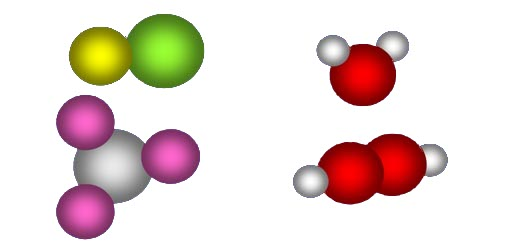
\includegraphics[width=40.0mm]{molecules.jpg} 
\end{frame}


\begin{frame}
	\begin{block}{Skipgrams}
		\begin{itemize}
			\item An n-gram with one or more gaps of specific length
			\item \emph{``to be *2* to be''}
			\item \emph{``ne *1* pas''}
		\end{itemize}
		\begin{center}
			 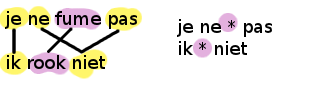
\includegraphics[width=50.0mm]{skipgram.png}
		\end{center}		
	\end{block}
\end{frame}


\begin{frame}
	\begin{block}{Research focus}
		``Constructions'' and their application in Machine Translation
	\end{block}

	\begin{block}{Stages of research}
		\begin{enumerate}
			\item Identification and extraction of constructions from monolingual corpus data 
			\item Alignment of constructions for a language pair (local translation step)
			\item Machine learning to map constructions in context (local translation step)
			\item Decoding (global translation step)
		\end{enumerate}
	\end{block}
\end{frame}



\section{Pattern detection}

\begin{frame}{Pattern detection}

	\begin{block}{Hypothesis}
		We can efficiently find constructions in large corpus data, limiting memory consumption
	\end{block}

	\begin{block}{Counting n-grams}
		\begin{itemize}
			\item Iterative counting, first unigrams, then bigrams, 
			\item  ... discarding pattern candidates if a sub-part is not found
		\end{itemize}
	\end{block}

	\begin{block}{Counting skip-grams}
		\begin{itemize}
			\item Counting constructions with gaps: \emph{``to be * to be''}
			\item ...by punching all combinations ``holes'' in found consecutive constructions
			\item ...discarding pattern candidates if consecutive sub-part is not found
		\end{itemize}
	\end{block}

\end{frame}

%\begin{frame}
%	\begin{block}{More about containing memory and scalability}
%		\begin{itemize}
%			\item Concise data representation
%			\begin{itemize}
%				\item Dynamic byte-size representation for all types in the corpus, longer representations for less occurring types
%			\end{itemize}
%			\item Occurrence thresholding
%		\end{itemize}
%		
%	\end{block}
%
%	\begin{block}{Pattern models}
%		\begin{itemize}
%			\item Indexed (most informed)
%			\item Unindexed (smaller memory footprint)
%		\end{itemize}
%	\end{block}
%\end{frame}

\subsection{Relations}

\begin{frame}
	\begin{block}{Relations}
		Extracted patterns/constructions can be related in various ways and represented in a \emph{graph model}
	\end{block}


	\begin{block}{Motivations}
		\begin{itemize}
			\item To make explicit the information contained in the relations
			\item Extra information may help in constraining to ``good'' constructions and help obtain good alignments
		\end{itemize}
	\end{block}

	\begin{example}
		``I see the dog move''
		\begin{itemize}
			\item \textbf{Subsumption:}   ``I'' is a sub-part of `'I see''
			\item \textbf{Succession:}	  ``see`` is a successor of ``I''
			\item \textbf{Instantiation:}   ``I see the dog move'' instance of ``I see *2* move''
		\end{itemize}
	\end{example}		
\end{frame}



%\begin{frame}{Subsumption relations}
%  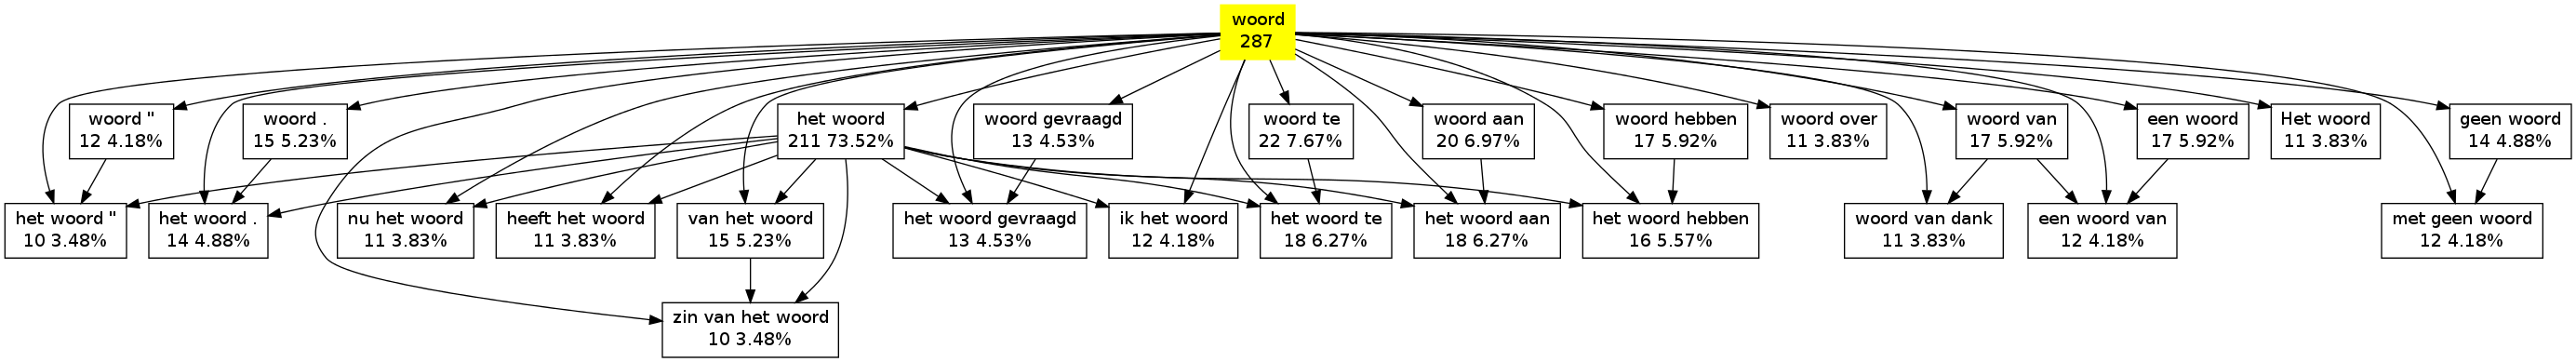
\includegraphics[width=160.0mm]{graph_woord_P.png}
%\end{frame}

%\begin{frame}{All relations: ``woord''}
% 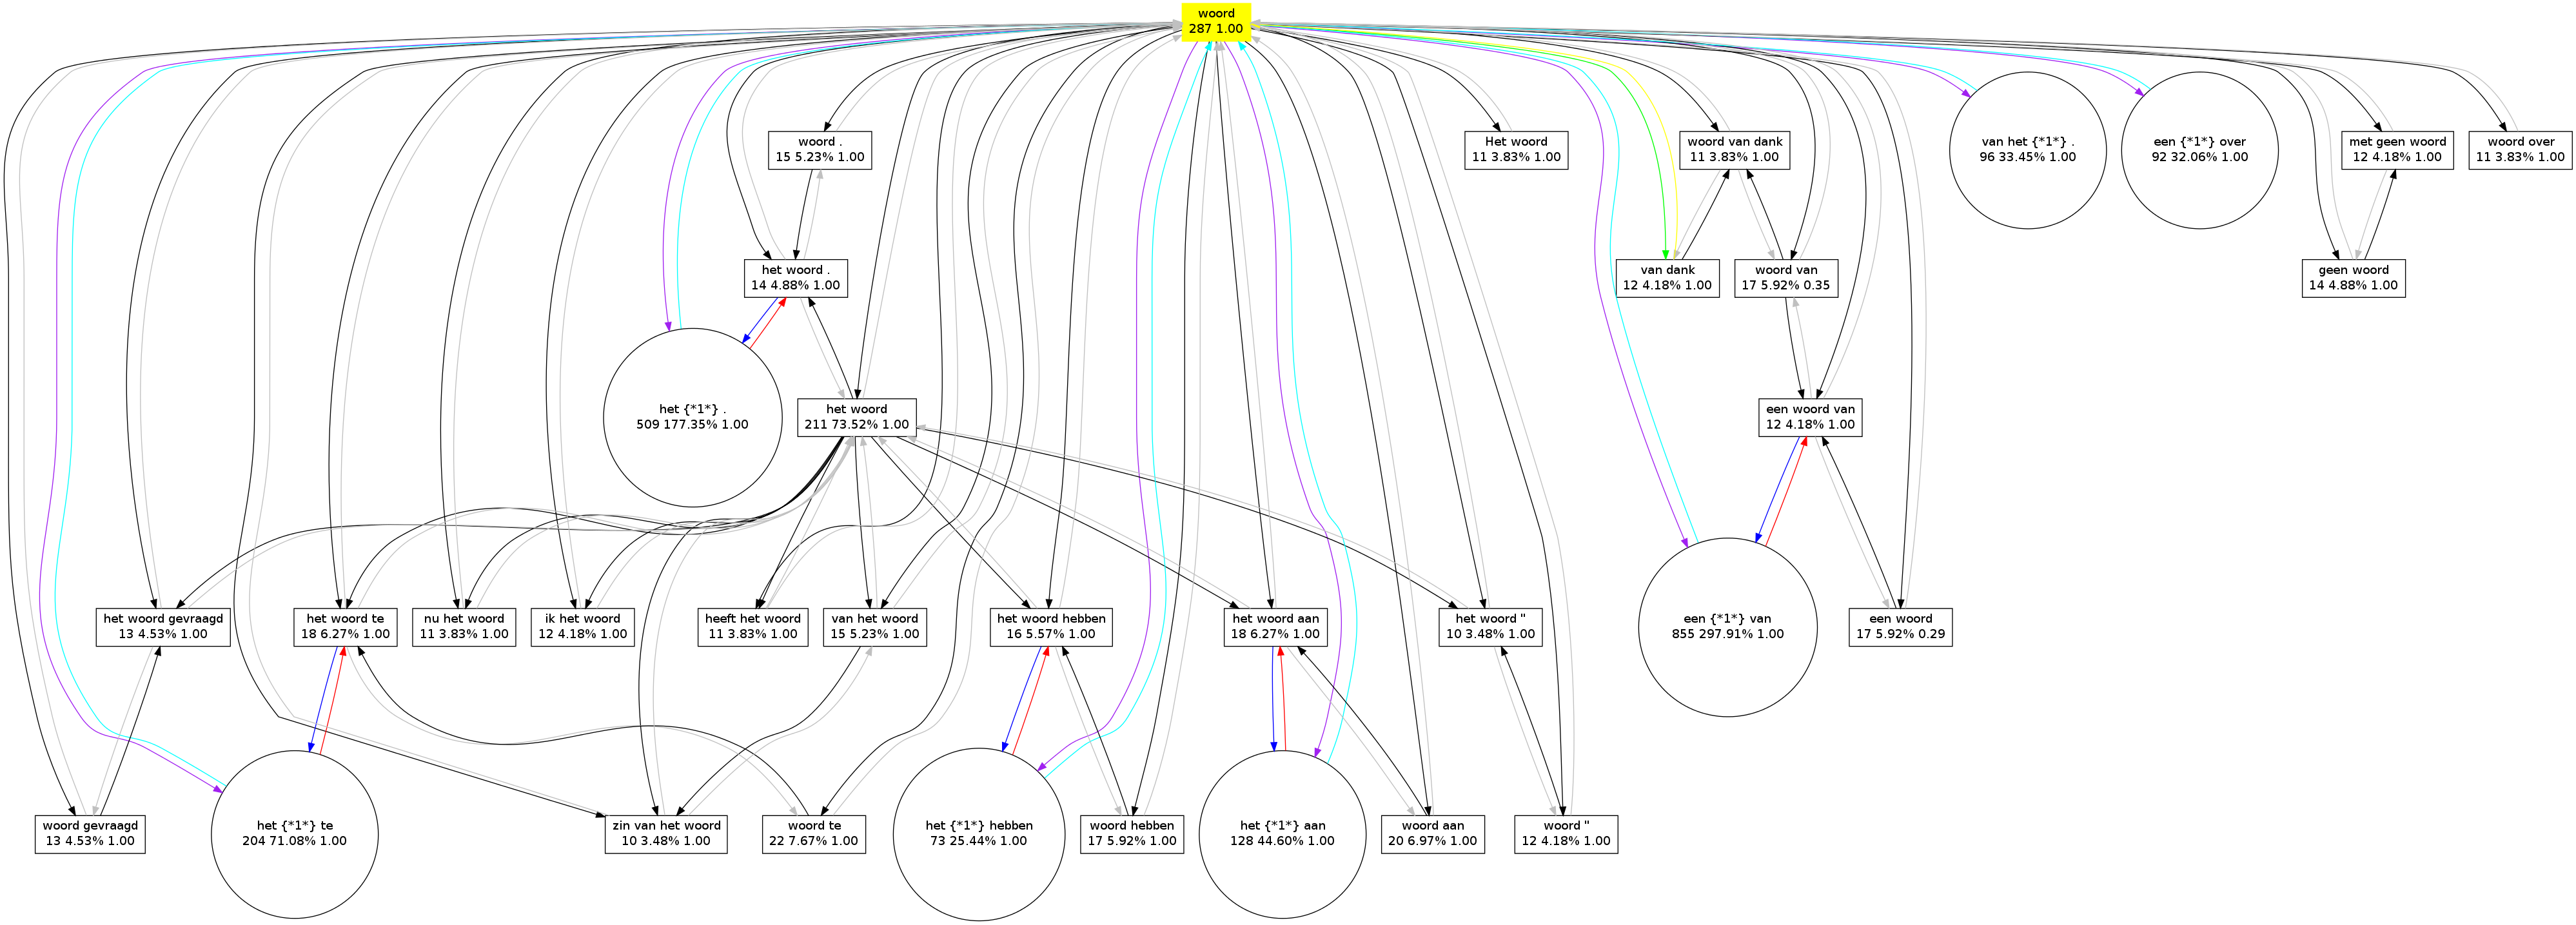
\includegraphics[width=170.0mm]{graph_woord_all.png}
%\end{frame}

\begin{frame}{All relations: ``tot $*$ van''}
 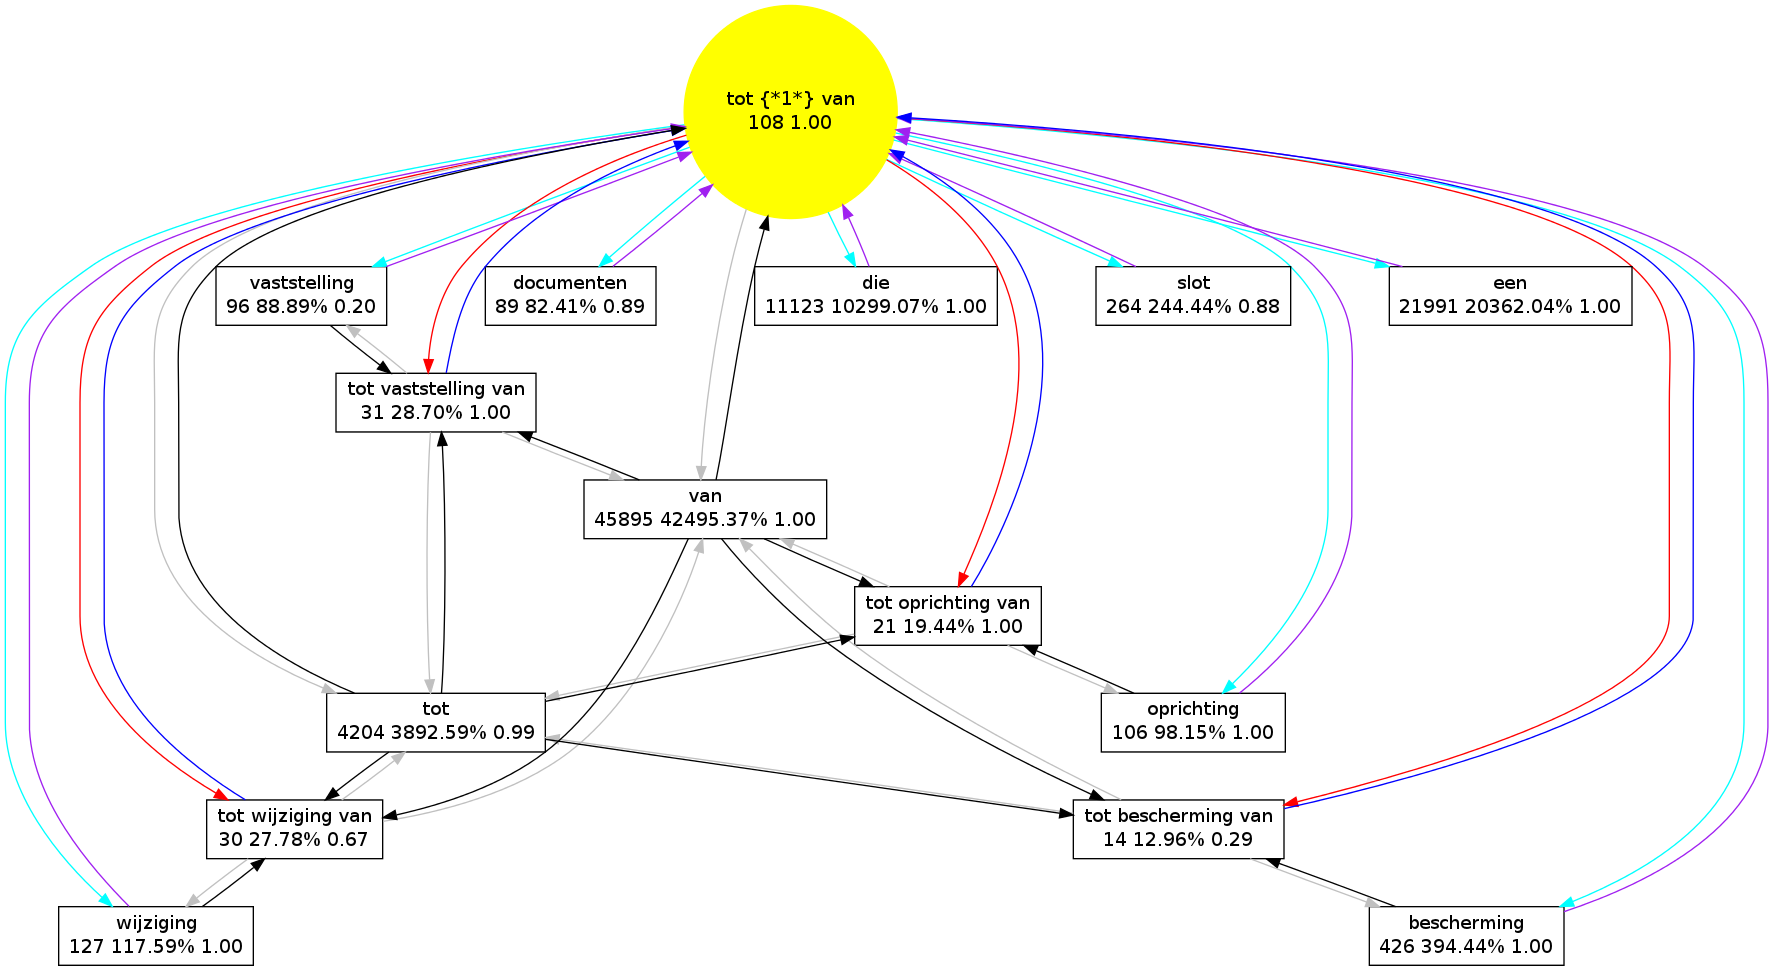
\includegraphics[width=140.0mm]{graph_totvan_all.png}
\end{frame}

\section{Alignment}

\subsection{Introduction}

\begin{frame}{Alignment}

	\begin{center}
	 
\includegraphics[width=45.0mm]{align1.png} 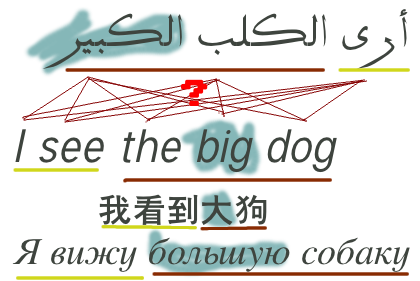
\includegraphics[width=45.0mm]{align2.png} 
	\end{center}

	\begin{block}{Goal}
		\textbf{Goal:} phrase-translation table
	\end{block}


	\begin{block}{Question}
		Can we align extracted patterns directly?
	\end{block}

\end{frame}

\subsection{Common method}

\begin{frame}
	\begin{block}{Common method in Phrase-based Statistical MT}
		\begin{enumerate}
			\item GIZA++ Word Alignment: source $\rightarrow$ target (IBM1, HMM, IBM4)
			\item GIZA++ Word Alignment: target $\rightarrow$ source
			\item Intersection of both
			\item Heuristic methods adding certain alignment points from the union (grow-diag-final) (Och and Ney, 2003)
			\item Extract all possible phrases
		\end{enumerate}
	\end{block}

\end{frame}


\begin{frame}{Alignment}
	 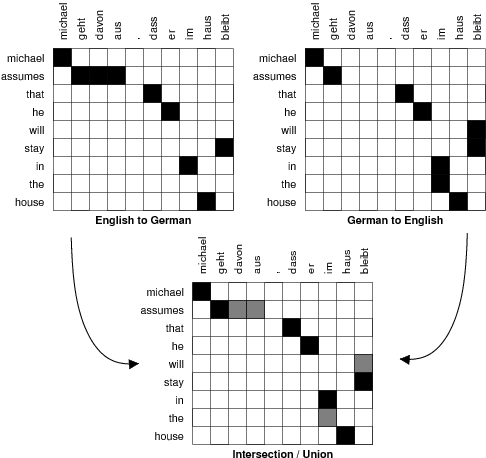
\includegraphics[width=80.0mm]{growdiagfinal.png}
\end{frame}

\subsection{Our method}

\begin{frame}
	\begin{block}{Intuitions}
		\begin{itemize}
			\footnotesize
			\item Word alignments are just an intermediate step towards phrasetables, we don't really need them.
			\item Word alignments introduce extra source for errors (poor quality alignments)
			\item Large memory availability might allow for more direct solutions
		\end{itemize}
	\end{block}
	\begin{block}{Our method}
		\begin{enumerate}
			\item Extract constructions for source language  
			\item Extract constructions for target language
			\item Attempt to directly align all constructions using EM (like IBM1):
			\begin{itemize}
				\item source $\rightarrow$ target
				\item target $\rightarrow$ source
				\item intersection
			\end{itemize}
			\item {\footnotesize Exploit graph-information (subsumption) to guide or adjust alignments}
		\end{enumerate}	
	\end{block}
\end{frame}

\begin{frame}
	\begin{block}{Graph information to aid alignment?}
		\begin{itemize}
			\item ... by pre-pruning constructions to include only ``exclusive'' constructions			
			\item ... by adjusting alignment weights (reward and punishment) based on subsumption relations
		\end{itemize}
		
	\end{block}
\end{frame}





\begin{frame}
	\begin{block}{Difficulties}
		\begin{itemize}
			\item Larger alignment matrix: larger memory consumption, scalability issues
			\item Competition of overlapping fragments? $\rightarrow$ skewed alignments
		\end{itemize}
	\end{block}

	\begin{block}{Preliminary results using Colibri alignment and Moses decoder (without skipgrams!)}
		\begin{itemize}
			\item Evaluations scores (BLEU etc) a bit below the classic approach ($+-$ 0.01 BLEU-points)
			\item But: significantly smaller phrase-table $\rightarrow$ more generalisation
			\item Graph information not helpful in alignment yet
		\end{itemize}
	\end{block}
\end{frame}




\section{Future}

\begin{frame}{Future}

	\begin{block}{Future \& Discussion}
		Alignment quality not sufficient yet..
		\begin{itemize}
			\item Reduce skewed alignments
			\item Scalability issues
			\item Graph information not helpful thus far, how to improve and integrate in EM?
		\end{itemize}

		Shifting focus to skipgrams...
		\begin{itemize}
			\item Alignment of skipgrams
			\item Development of an MT decoder that supports skipgrams
		\end{itemize}
	\end{block}
\end{frame}


\begin{frame}

\raccoon

\begin{center}
\Large{Questions?}
\end{center}

\end{frame}

\section{Extra}



\begin{frame}{MT Pipeline}
	\begin{center}
	 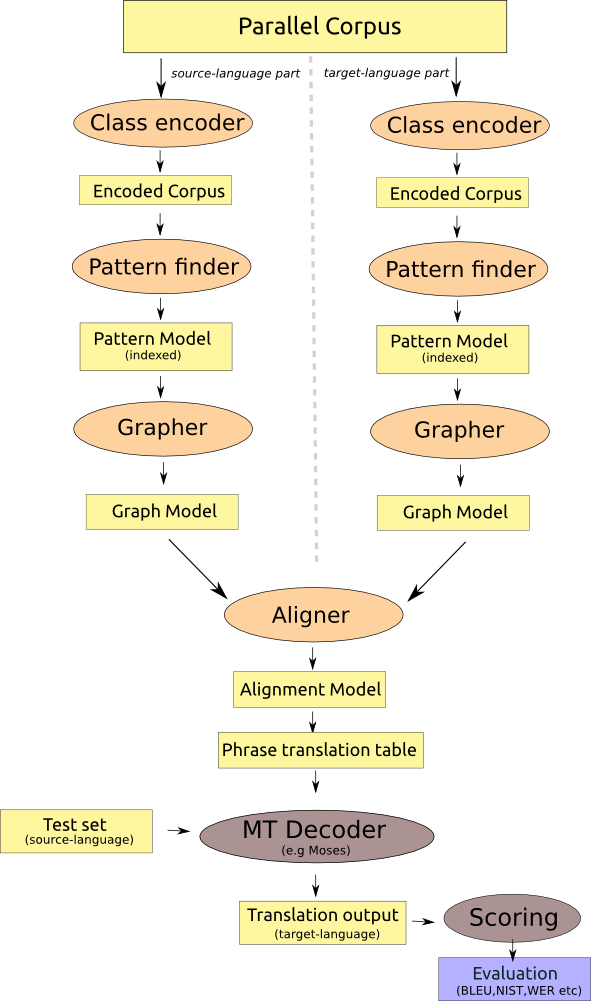
\includegraphics[width=40.0mm]{colibri_mtarch.png}
	\end{center}
\end{frame}






\begin{frame}[fragile]{IBM Model 1 EM}
\footnotesize
\begin{lstlisting}[python]
initialize t(t|s) uniformly
do until convergence
  set count(t|s) to 0 for all t,s
  set total(s) to 0 for all s
  for all sentence pairs (t_s,s_s)
     set total_s(t) = 0 for all t
     for all patterns t in t_s
        for all patterns s in s_s
          total_s(t) += t(t|s)
     for all patterns t in t_s
         for all patterns s in s_s
            count(t|s) += t(t|s) / total_s(t)
            total(s)   += t(t|s) / total_s(t)
  for all s
 	for all t
       t(t|s) = count(t|s) / total(s)
\end{lstlisting}
\end{frame}




\end{document}
